%\documentclass[10pt,twoside,a4paper]{book}
\documentclass[10pt,twoside,a4paper,twocolumn]{book}
%\documentclass[10pt,twoside,a4paper,titlepage,draft]{book}

\usepackage{mystyle}

%\includeonly{mathematics/logic.and.proof/logic.and.proof}

\begin{document}
\begin{titlepage}
\begin{center}
\hrule
{ \huge \bfseries PHYSIC\AE\\  MATHEMATICA}\\[0.5cm]
\hrule
The Philosophy of Mathematics and Physics

\emph{Collaborators:}\\
\begin{tabular}[center]{ccr@{@}l}
    Michael Schmidt & University of Colorado at Boulder & Michael.Schmidt & Colorado.EDU\\
    %Bryan Kaufman & University of Colorado at Boulder & Bryan.Kaufman & Colorado.EDU \\
\end{tabular}

\begin{figure*}[!h]
    \centering
	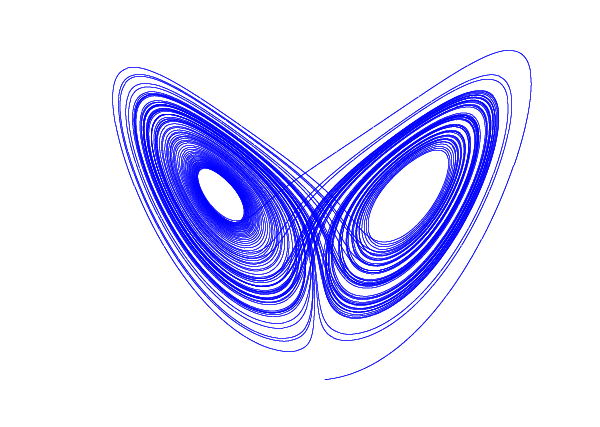
\includegraphics[scale=0.60]{./attractor.png}
\end{figure*}

\vfill
{\large \today}\\

This project is freely available at:\\
\url{http://github.com/schmidmt/Physicae-Mathematica}

\end{center}

\vfill


\end{titlepage}

%$Id: coverdetails.tex 6 2009-04-23 02:25:09Z schmidmt $%

\begin{center}
\begin{verbatim}
	Copyright (C)  2009 Michael Schmidt.
	Permission is granted to copy, distribute and/or modify this document
	under the terms of the GNU Free Documentation License, Version 1.3
	or any later version published by the Free Software Foundation;
	with no Invariant Sections, no Front-Cover Texts, and no Back-Cover Texts.
	A copy of the license is included in the section entitled "GNU
	Free Documentation License".
\end{verbatim}
\end{center}


\begin{center}
	\emph{Thanks To:}
\end{center}


\phantomsection
\tableofcontents

\subsection*{Preface}
\addcontentsline{toc}{subsection}{Preface}
	\indent
	I began writing this book while attending the University of Colorado at Boulder.
	I'm writing this to help solidify my understanding of physics.
	My idea is if I am able to explain the concepts and mathematics behind physical theories then I understand them myself.
	This is not meant to be an introduction but simply a review of what is covered in an undergraduate curriculum.
	Hope you enjoy.\\
	\begin{flushright}
	%\Fontauri{{Michael Schmidt}}
		-Michael Schmidt\\
	\end{flushright}


\part{Mathematics}
\startsoln
\chapter{Introduction}
    \begin{quote}
        Mathematicians are people who would rather think than work.\newline
        \flushright{--David Grant}
    \end{quote}

    \bigskip

    First we shall start off with a definition:
    \begin{defn}
       \index{Abstraction}
       \underline{\emph{Abstraction}} is the process of producing a concept not associated with a specific instance.
    \end{defn}
    Why do we want this?
    Well it's simple, we would like to figure out how to build up concepts to permit us to predict, discover, and create new ideas.
    By grouping specific instances into concepts we can apply what we learn to a plethora of instances not just one.
    Also, we can use what other people have thought of and apply it to another instance without redoing the thinking.
    Besides, by abstracting we may discover new ideas which we could have never discovered otherwise.
    
    This brings us to our first main topic, mathematics.
    Mathematics is a philosophy used to bring together a vast number of topics into one topic so similarities between ideas may be exploited to discover the most elegant solution.
    For instance, ideas from calculus can be applied to geometry to analyze how shapes are, for lack of a better word, shaped.
    In regards to the quote above, math is a tool used to prevent "brute forcing" a solution.
    By "brute forcing" I mean trying every since possibility, basically guess and check with no direction at all.
    That would talk too much time.
    Remember if we can figure out a way to think of an problem in the most abstract we can more easily figure out the best way to solve it.

    So we start our endeavor first by ascertaining an idea of how to connect ideas.
    This topic is what we have come to call logic.

    \lipsum

\chapter{Logic and Proof}

\nocite{Richmond2004Discrete}

\section{Logic}

So we start our discussion of logic with an idea.
Now ideas can be seen to have two distinct values of validity: true and false.
We refine these ideas into a statement, which is defined as follows:

\begin{defn}
	\index{Statement}
	A \underline{\emph{statement}} is a phrase which is either true or false. (A statement can be represented by a letter for simplicity and compactness.)
\end{defn}

So a statement encompasses an entire idea and can be evaluated to determine its validity

\begin{ex}
    For instance we have the following statements:
	\begin{center}
    P="The sky is blue".\\
	Q="The sky is brown".
    \end{center}
    We see the statement P is \emph{True} while the statement Q is \emph{False}.
\end{ex}

So what if our statement is simply the opposite of another statement, how can we easily represent it?
We have invented notation for this exact purpose, it is called the negation and is defined like so:

\begin{defn}
	\index{Negation $\neg$}
	\nomenclature{$ \land $}{Logical And. True if all elements are true and false otherwise.}
	The \underline{\emph{Negation}} ($\neg$) of a statement is true when the statement is false and false if the statement is true.
	(The statement $\neg P$ is written in other words as "Not P".)
\end{defn}

\begin{ex}
    Using the examples above:
    \begin{center}
	$\neg P=$"The sky is not blue".\\
	$\neg Q=$"The sky is not brown".
    \end{center}
    Here $\neg P$ is \emph{False} and $\neg Q$ is \emph{True}.
\end{ex}

\subsection{And and Or}
So far we have only been able to create very simple statements, but what if we want to combine multiple statements into a larger statement?
We can combine them using connectives \emph{and} and \emph{or}.
Since in language these two words are defined very vaugely, we will give them exact definitions so they may be used precisely.

\begin{defn}
	\index{And, Logical $\land$}
	\nomenclature{$ \lor $}{Logical Or. True if any elements is true and false otherwise.}
	A \underline{\emph{conjunction operator}}, or "And" ($\land$), connects logical statements which is defined to be true if all statements are true and false if any are false.
\end{defn}

To help better understand how these operators work we use a table which places all possible inputs with their corresponding outputs in a table.
This table is then called a truth table where the two possibilities are true(T) and false(F) for every field.
The truth table for the conjunction operator is as follows:

\begin{center}
	\begin{tabular}{cc|c}
		$P$ & $Q$ & $P \land Q$ \\
		\hline
		T & T & T \\
		T & F & F \\
		F & T & F \\
		F & F & F \\
	\end{tabular}
\end{center}

So what happens if we take the negation of the statement $P \land Q$?
Well, the statement says, "Not both P and Q", which can be interpreted as "neither P nor Q", which again can be rewritten as "Not P or Not Q".
Using this idea or an \emph{or} connective we can define the disjunction operator as follows:

\begin{defn}
	\index{Or, Logical $\lor$}
	A \underline{\emph{disjunction operator}}, or "Or" ($\lor$), connects logical statements and is true if any statements are true and false if all are false.
\end{defn}

So lets look at the truth table for the disjunction operator with the conjunction operator.

\begin{center}
	\begin{tabular}{cc|ccc}
		$P$ & $Q$ & $P \land Q$ & $P \lor Q$ & $\neg P \lor \neg Q$ \\
		\hline
		T & T & T & T & F \\
		T & F & F & T & T \\
		F & T & F & T & T \\
		F & F & F & F & T \\
	\end{tabular}
\end{center}

From this we can see that $\neg (P \land Q)$ is equivalent to $\neg P \lor \neg Q$.
We can also look at the negation of the statement $P \lor Q$ by looking at it as the sentence, "Not either P or Q", and the only time that will work is when both P and Q are false, so the sentence becomes, "Not P and Not Q".
This can be rewritten as $\neg P \land \neg Q$.
This brings us to our first theorem, originally stated as laws by De Morgan.

\begin{thm}
	\index{De Morgan's Laws (Logic Version)}
	\textbf{(De Morgan's Laws)} \\
	\label{Thm:DeMorganLogic}
	\begin{equation}
		\nonumber
		\neg ( P \land Q ) \iff \neg P \lor \neg Q
	\end{equation}
	\begin{equation}
		\nonumber
		\neg ( P \lor Q ) \iff \neg P \land \neg Q
	\end{equation}
\end{thm}
Here the symbol $\iff$ means logically equivalent, we will generalize its meaning to "if and only if" operator later in the chapter.

\begin{proof}
	To prove theorem \ref{Thm:DeMorganLogic} we can construct the truth tables for the statements involved relatively simply.
	\begin{table*}[ht]
	\begin{center}
	\begin{tabular}{cc|cc|cccccc}
			$P$ & $Q$ & $\neg P$ & $\neg Q$ & $P \land Q$ & $\neg (P \land Q)$ & $P \lor Q$ & $\neg (P \lor Q)$ & $\neg P \lor \neg Q$ & $\neg P \land \neg Q$ \\
			\hline
			T & T & F & F & T & F & T & F & F & F \\
			T & F & F & T & F & T & T & F & T & F \\
			F & T & T & F & F & T & T & F & T & F \\
			F & F & T & T & F & T & F & T & T & T \\
	\end{tabular}
	\end{center}
	\end{table*}
	Since there are only four possible inputs for these operators, all possibilities have been shown and the theorem is proved.
\end{proof}

\begin{thm}
	\textbf{Properties of Logical Operators}\\
	\label{thm:proplogical}
	\textbf{Distributivity}: $(A \land B) \lor C \iff (A \lor C) \land (B \lor C)$ and $(A \lor B) \land C \iff (A \land C) \lor (B \land C)$
	
\end{thm}

\subsection{Implication}
We are ultimately concerned with using logic to show how two idea are connected.
Usually this connectedness is expressed in the form of a conditionals of the form, "If \emph{something} then \emph{something else}."
In terms of logic when a true statement causes another to also be true an implication is formed.
We can now define the implication as follows:

\begin{defn}
	\index{Implication, $ \Rightarrow $}
	An \emph{\underline{implication}} ($A \Rightarrow B$) between means that if A is true, so must B.
\end{defn}
With this definition, if A is false then B is unrestricted and can be anything.
So if A is false, the statement will always be true since a false statement implies anything.
We also note that if A is true but B is false, that would suggest that A doesn't imply B, so the statement is false.
Using this we can construct a truth table for an implication.

\begin{center}
	\begin{tabular}{cc|c}
		$P$ & $Q$ & $P \Rightarrow Q$ \\
		\hline
		T & T & T \\
		T & F & F \\
		F & T & T \\
		F & F & T \\
	\end{tabular}
\end{center}

So if $A \Rightarrow B$ is true, then a false B would imply a false A.
This brings us to the definition of the contrapositive.

\begin{defn}
	\index{Contrapositive}
	Given $A \Rightarrow B$, $\neg B \Rightarrow \neg A$ is called the contrapositive of $A \Rightarrow B$.
\end{defn}


\begin{exe}
    TEST
    \begin{soln}
        TEST1
    \end{soln}
\end{exe}

\section{Proof}

\subsection{Direct Proof}
\subsection{Proof By Contradiction}
\subsection{Proof By Induction}


\lipsum


\begin{bibunit}
    \putbib
\end{bibunit}

\chapter{Relations}

\lipsum

\chapter{Group Theory}

\chapter{The Numbers}


\chapter{Linear Algebra}

\chapter{Calculus}

\chapter{Complex Analysis}

\chapter{Ordinary Differential Equations}

\section{1st Order}

\section{2nd Order}

\section{Systems of 1st Order Differential Equations}



\chapter{Differential Geometry}

\chapter{Fourier Analysis}

\chapter{Partial Differential Equations}

\chapter{Numerical Analysis}

\lipsum



\part{Physics}
\chapter{General Statements}
    \begin{bibunit}
	\section{Noether's Theorem: Conservation Laws}

\label{sec:noether}
\begin{thm}
	For every symmetry there corresponds a conserved quantity.\cite{Noether2005Invariant}\index{Noether's Theorem}
\end{thm}
\lipsum

	\section{Lagrangian and Hamiltonian Dynamics}


	\putbib
	\end{bibunit}

\chapter{Classical Mechanics}
	\section{Introduction}
	Classical Dynamics Introduction...
	
	\section{Lagrangian and Hamiltonian Dynamics}

\lipsum

	\section{Newtonian Dynamics}
	\begin{equation}
		\vect{F} = \frac{d}{d t} (m \vect{v}) = \dot{\vect{P}}
		\label{Newton's Force equation}
	\end{equation}


	

\chapter{Electrodynamics}

\lipsum

	

\chapter{Quantum Dynamics}

\lipsum

\chapter{Plasma Physics}

\lipsum

\chapter{Particle Physics}

\lipsum

\chapter{Computational Physics}

\lipsum


\stopsoln

\part{Reference}

\appendix
\chapter{Solutuons}
%\addcontentsline{toc}{Section}{Solutions}
\putsoln

\onecolumn
\chapter{GNU Free Document License}
\verbatiminput{appendixes/fdl-1.3.txt}

\twocolumn

\addcontentsline{toc}{Section}{List of Figures and Tables}
\listoffigures
\listoftables

\addcontentsline{toc}{Section}{Symbols and Nomenclature}
\printnomenclature


\addcontentsline{toc}{Section}{Index}
\printindex

\end{document}
